\section{Indledning} 

Verden er mere og tættere forbundet end nogensinde; men også mere
polariseret. Vi befinder os i en brydningstid, hvor der i
stigende grad savnes samfundsmæssig konsensus om en 'facit'
omkring, hvordan verden arter sig og vi skal agere i den. Vi
samles omkring forskellige konstellationer af verdensopfattelser,
for at opnå en fornemmelse af tilhørighed blandt
meningsfæller \autocite{sulerUniqueGroupsCyberspace1999}.

Internettet gør det muligt, at finde dette fællesskab og denne
samhørighed på nye måder. Marginaliserede individer kan finde
sammen, upåagtet geografi, og deler frit og åbent erfaringer med
hinanden \autocite[s. 184]{sulerOnlineDisinhibitionEffect2004}. 
Der dannes positioner, hvor rettigheder, friheder, ansvar og
pligter forhandles i en evigt regenererende diskurs \autocite[s.
22]{harrePositioningTheoryMoral1999}.

Opleves der, at nogen siger det verdensbillede man har
internaliseret i mod, kan dette kan være meget svært at acceptere.
Man oplever, at ens selvopfattelse og selvbillede krænkes. Den
position man har antaget ikke altid bliver anerkendt af andre,
eller at man ikke vil anerkende den position, andre forsøger at
placere en i \autocite[s 30]{harrePositioningTheoryMoral1999}.

De samme processer der gør, at mennesker kan tillade sig at være
mere sårbare og ærlige online, er dog også til grund for meget af
den grove tone man hurtigt finder på de sociale medier. Denne 
ondartede udgave af online disinhibition betyder, at der ikke skal
meget til, før miljøet online hurtigt bliver giftigt
\autocite{sulerOnlineDisinhibitionEffect2004}.

Derudover har internettet bidraget med nye settings for at vise 
hvem man \sout{vil fremstå som at være} er. De sociale medier 
giver os nye rammer for sociale interaktioner, og nye scener for 
fremvisning af de roller vi ønsker at blive identificeret ved.

Jeg vil undersøge, hvordan disse processer arter sig på sociale
medier. Konkret vil jeg tage Instagram som præsentation- og
positionsarena for mig, og se på hvordan selvpræsentationer 
bidrager til positionering omkring emnet maskulinitet.

Det følgende afsnit vil præsentere mit teoretiske grundlag for
denne undersøgelse. Derefter vil jeg introducere mit konkrete
fokusområde, med en efterfølgende kort gennemgang af undersøgelser
med et lignende fokus.

Herefter vil jeg drøfte mit empiriske analysegrundlag, med
tilhørende diskussion af mulige analyseresultater. Afslutningsvis
vil jeg diskutere og perspektivere mine konklusioner i et bredere
sociologisk perspektiv.

\section{Teoretisk analysegrundlag}

Jeg tager primært udgangspunkt i en positionsteoretisk tilgang, 
som beskrevet af \citeauthor{harrePositioningTheoryMoral1999}.   
Denne særlige, situerede diskursanalyse 
\autocite{harreRecentAdvancesPositioning2009} bliver suppleret med
bemærkninger fra 
\citeauthor{goffmanPresentationSelfEveryday1956}, hvor jeg 
anvender teatermetaforen præsenteret i 
\citetitle{goffmanPresentationSelfEveryday1956} 
(\citeyear{goffmanPresentationSelfEveryday1956}), på den 
formidling af “selv” der foregår på Instagram.  John Suler
bidrager med en cyberpsykologisk forståelse af, hvordan 
udbredelsen af cyberspace påvirker den menneskelige selvforståelse
og kommunikationsstrategier.

\subsection{Positioneringsteori}

\citeauthor{harrePositioningTheoryMoral1999} beskriver 
positioneringsteori som (\citeyear[s. 1, min oversættelse
]{harrePositioningTheoryMoral1999}):
\begin{quotation}
  \ldots studiet af lokale morale ordener som evigt skiftende 
  mønstre af gensidige og omtvistelige rettigheder og 
  obligationer af tale og handlen \ldots
\end{quotation}

Positioner påvirker dermed hvordan og hvorledes individuelle 
handlemåder og handlemuligheder. Er man positioneret som uvidende 
om et emne, tildeles man ikke ret til at bidrage til diskussioner 
herom. Derudover er positioner generelt set relationelle, idet at 
nogen må indtage positionen “magtesløs” for at andre kan have 
positionen “mægtig”.

Positioneringsteori vil undersøge, hvordan diskursive processer 
producerer psykologiske fænomener. Den tager udgangspunkt i, at 
vores oplevede liv brydes op til \emph{episoder} i gennem 
diskurser. Det er disse episoder, der er grundlaget for både vores
livshistorier og den sociale verden \autocite[s. 
4]{harrePositioningTheoryMoral1999}.

Episoder i denne kontekst omfatter “enhver serie hændelser hvor 
mennesker deltager, hvor der er en form for enhedprincip”. De 
indbefatter, ud over synlig adfærd, også deltagernes tanker, 
følelser, intentioner med mere. De både former deltagernes 
handlinger, og er definerede af dem \autocite[s. 
5]{harrePositioningTheoryMoral1999}.

Hvor en positioneringsteoretisk analyse skiller sig fra for 
eksempel en interaktionsanalyse på baggrund af 
\citeauthor{goffmanPresentationSelfEveryday1956} i
\citetitle{goffmanPresentationSelfEveryday1956}, er et explicit 
fokus på situationens historicitet. Episoder bliver til på 
baggrund af foregående episoder, og vil indeholde elementer der 
ikke kan forklares på baggrund af generelle regler og roller 
\autocite[s. 5-6]{harrePositioningTheoryMoral1999}.

Dermed fremhæves tre grundlæggende egenskaber af, hvordan sociale 
og psykiske fænomener konstrueres 
\autocite{harrePositioningTheoryMoral1999}:
\begin{enumerate}
  \item
    deltagernes morale positioner, og tilhørende ret og pligt 
    til bestemte ytringer
  \item
    samtalens historik
  \item
    de faktiske udsagn, med kraft til at give form til dele af 
    den sociale verden
\end{enumerate}

\subsubsection{Positioneringens forståelsesramme}

Indenfor positioneringsteorien anses mennesker for at være 
placeringer for sociale handlinger, hvor 'samtalen' er den 
grundlæggende bestanddel af den sociale verden. Der er i samtalen,
den sociale verden bliver skabt; og sociale handlinger genereres 
og reproduceres \autocite[s. 
15]{harrePositioningTheoryMoral1999}.

I denne forståelse af den sociale verden som bestående af 
\emph{personer} og \emph{samtaler}, er positionering en “\ldots 
diskursiv konstruktion af personlige fortællinger, der gør en 
persons handlinger forståelige og relativt fastgjorte som sociale 
handlinger, og hvori samtalens medlemmer har specifikke 
placeringer.” \autocite[s. 16]{harrePositioningTheoryMoral1999}

Dermed er positioner i en samtale en samling af personens moralske
og personlige egenskaber. Man kan positionere sig — eller blive 
positioneret — som mægtig eller magtesløs, selvsikker eller 
undskyldende, med videre. En handlings sociale gennemslagskraft og
deltagernes positioner er videre forbundne, idet samtaler har 
historier, og de positioner der indtages i en samtale er forbundne
med disse historier. Der er dermed en gensdigt skabende triade, 
bestående af følgende elementer \autocite[s.  
17-18]{harrePositioningTheoryMoral1999}:


\begin{figure}[!h]
\label{fig:triad}
\centerline{
  % Resize it to 5cm wide.
  \resizebox{7cm}{!}{
    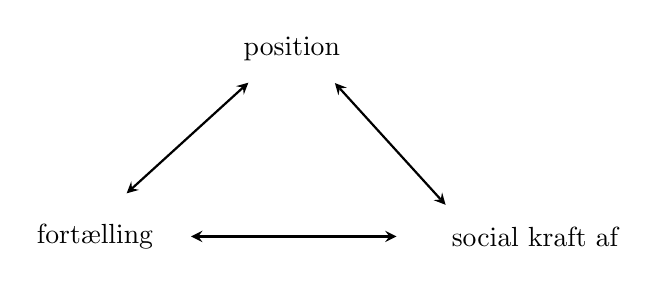
\begin{tikzpicture}[
      scale=0.5,
      trans/.style={thick,<->,shorten >=2pt,shorten 
      <=2pt,>=stealth},
    ]
    \draw[trans] node {fortælling} (0.7,1) -- (4,4) node[above, 
    xshift=0.5cm, yshift=0.1cm] {position};
    \draw[trans] (6,4) -- (9,0.7);
    \draw[trans] (2.3,0) -- (7.8,0) node[right, xshift=0.5cm] 
  {social kraft af}; \end{tikzpicture}
  }
}
\caption{De tre gensidigt afhængige elementer i en situation}
\end{figure}


Positioner kan opstå “naturligt” i situationen; men en besiddelse 
af den dominerende rolle i en samtale vil kunne tvinge de andre 
talere i positioner de ellers ikke ville have indgået frivilligt.  
Dog kan disse begyndende positioner anfægtes, og talerne dermed 
blive ompositionerede \autocite[s. 
18]{harrePositioningTheoryMoral1999}. Disse “naturligt” 
forefindende positioner er selv produkter af  positionshandlinger
af højere ordener, hvor rettigheder og  pligter til at tillægge
eller modstå positioner distribueres  \autocite[s.  
8]{harreRecentAdvancesPositioning2009}.

Ved at starte en samtale af en højere orden, hvor den foregående 
samtale blot er et emne, kan man positionere sig som kommentator 
på positioner, historier og sociale handlinger deri \autocite[s.  
18]{harrePositioningTheoryMoral1999}. Videre kan den samme 
historie være del i flere narrativer, der foregår sideløbende,  og
have forskellige  betydninger i hvert narrativ 
\autocite{harreRecentAdvancesPositioning2009}.

Positioneringsteorien ser dermed på hvordan mennesker opfører sig 
overfor hinanden, og forsøger at afdække de implicitte og 
eksplicitte tankemønstre der ligger til grund for dette 
\autocite[s. 5]{harreRecentAdvancesPositioning2009}.
Fokus er dermed ikke på et direkte kausalitetforhold mellem social 
handlinger; men derimod på de meningsforhold der forbinder dem.  
Disse meningsforhold springer ud af en lokal kanon af normer og 
regler, og er også med til, at mediere forholdet mellem bærere af 
specifikke medier \autocite[s. 
7]{harreRecentAdvancesPositioning2009}.

\subsection{Selvets præsentation}

I den førnævnte \citetitle{goffmanPresentationSelfEveryday1956} 
beskriver \citeauthor{goffmanPresentationSelfEveryday1956} hvordan 
mennesker præsenterer forskellige facetter af sig selv i 
forskellige sammenhænge. “Selvet” er i denne forståelse 
relationelt, og er afhængigt af, at de personer individet 
interagerer med i en given situation anerkender den \emph{persona} 
individet har antaget i en given situation, og dermed også 
individets moralske ret til at blive behandlet på en bestemt måde 
\autocite[s.  6-7]{goffmanPresentationSelfEveryday1956}.

\citeauthor{goffmanPresentationSelfEveryday1956} anvender en 
teatermetafor gennemgående i sin analyse. De forskellige personaer 
bliver i denne sammenhæng kaldt \emph{roller}, og de andre 
deltagere i en situation (hvad i en positionsanalyse vil være en 
episode) bliver tilskuere til en præsentation. Samtidig spiller 
disse tilskuere selv en rolle, og vi er på denne måde alle 
hinandens tilskuere \autocite[s. 
???]{goffmanPresentationSelfEveryday1956}.

Dette relationelle selv individet præsenterer vil, i følge 
\citeauthor{goffmanPresentationSelfEveryday1956} være et 
idealiseret selv. Individet vil ikke være i besiddelse af alle de 
kvaliteter, der er forventet af rollen, men forsøger at leve op 
til disse alligevel (\citeyear[s.  
?]{goffmanPresentationSelfEveryday1956}). Individet vil dermed 
forsøge konstant at bedrive “impression management”, for at 
henlede opmærksomheden væk fra, de områder hvor det ikke er 
opnåeligt, at leve op til rollens krav. Samtidig vil tilskuerne 
anvende pli og høflighed, for ikke at gøre opmærksom på, at der er 
sket et fejltrin \autocite[s.  
7-8]{goffmanPresentationSelfEveryday1956}.

For at kunne opretholde en social front, taler 
\citeauthor{goffmanPresentationSelfEveryday1956} om 
\emph{settings}, der udgør den scenografiske del af en optræden, 
samt \emph{udseende} (der giver os indblik i individets sociale 
status) og \emph{opførsel} (der kan fortælle os, hvilken rolle 
individet forventer at indtage).  Der er ofte en forventning om, 
at der er et vist samsvar mellem setting, udseende og opførsel 
\autocite[s. 14-15]{goffmanPresentationSelfEveryday1956}.

Optrædener foregår gerne i en afgrænset \emph{region}, og kaldes 
af \citeauthor{goffmanPresentationSelfEveryday1956} \emph{front
region}. Der foretages en analytisk sondring mellem  denne
frontregion, hvor rollen udleves; og regionen  \emph{backstage},
hvor rollen kan lægges væk, og individet kan få  afløb for de
sider af sig selv, der ikke er forenelig med rollen  (\citeyear[s.
69]{goffmanPresentationSelfEveryday1956}).

\section{Instagram som positionerings- og præsentationsarena}

Instagram er et socialt medie bygget op omkring offentliggørelse 
af billeder og korte videoklip. \footnote{Der er dog mulighed for,
at opretholde en privat profil på Instagram, hvor man skal 
godkendes som følger af en bruger for at se vedkommendes 
billeder.} Medlemmer kan “følge” andre brugere, for at inddrage 
disse brugeres billeder med i sin nyhedsstrøm af billeder. De 
publicerede billeder kan suppleres med en billedtekst, der ofte 
indeholder \texttt{\#hashtags}.  Disse hashtags samler flere 
billeder omkring et emne — til en samtale, om man vil. Hashtags 
gør det også muligt for billeder at nå frem til andre der er 
interesserede i samme emne, uden at disse brugere aktivt følger 
personen, der lagde billedet op. Dette kan både ske aktivt; ved at
følge en bestemt hashtag, eller passivt, ved at Instagrams 
algoritmer foreslår opslag.

Når det sociale ses som bestående af personer og samtaler, er der 
her mange samtidige samtaler at gribe fat i med et 
positioneringsteoretisk blik. Selve billedet er et bidrag til en 
samtale. Derudover er billedtekst og tilhørende hashtags med til, 
at vise hvilken position der indtages omkring et bestemt emne — 
og, qua den iboende relationelle kvalitet i positioneringen, 
hvilke positioner der konstrueres for ens “modstandere” omkring 
dette emne. Og billedteksten er for en social ytring at regne - 
der har (potentiel) kraft til at forme den sociale verden.

Men den sociale positionering er ikke kun indbefattet i den 
konkrete ytring. Udvælgelse af hashtags, og de fællesskaber man 
dermed henvender sig til og (dis)associerer sig med, er også en 
form for social talehandling, der påvirker og forholder sig til en 
social fortælling — og ikke nødvendigvis den samme, som billede og 
billedtekst.

Det er her vigtigt, at holde øje på, at en talehandling kan yde 
indflydelse på to måder: hvad der opnås, i at sige noget — 
kommentaren “Sådan!” signalerer, at noget er en bemærkelsesværdig 
præstation; og hvad der opnås ved at sige noget — her, at glæde 
den præsterende part \autocite[s. 
17]{harrePositioningTheoryMoral1999} 

\subsection{Selvudstillelse eller selvskabelse?}

Ville man have spurgt 
\citeauthor{goffmanPresentationSelfEveryday1956} om hans holdning 
til ovenstående spørgsmål, ville han formentlig kigget uforstående 
tilbage. For ham var de to ting uløseligt sammenbundne. Ved at 
udstille sig som det “selv” individet ønsker at fremstå som, 
skaber individet en opfattelse af sig som dette “selv”.

Instagram er, i teatermetaforen, en en særlig form for performativ 
scene, hvor man har gode muligheder for at styre andres 
opfattelser af en selv. Det er muligt, at holde en skarp 
adskillelse af front- og backstage, hvor det online publikum ikke 
får adgang til rollens konstruktion. Individet har videre god 
kontrol over de sceniske aspekter af sin optræden, og kan styre de 
sociale tegn der formidles igennem rekvisitter med videre. 

En af de mest fremtrædende forskere i sociale mediers betydning
for individer er den amerikanske psykoanalytiker John Suler. 
\citeauthor{sulerSelfPortraitsSelfies2015} har set på, hvordan 
mennesker iscenesætter sig selv online via selvportrætter — 
“selfies”. Instagram består ikke kun af selfies. Men den generelle 
idé, der peges på, kan overføres til andre billeder der 
distribueres på sociale medier som en del af selv-præsentation og
kontrol af andres indtryk af ens (aktuelle) selv. Det er en
effektiv måde, at løfte sløret for sig “selv”, samtidig med, at
man forsøger at styre denne fremvisning af selvet 
(\citeyear{sulerSelfPortraitsSelfies2015}).

På Instagram kan andre brugere give ens opslag et 'like', hvor der 
tilkendegives en form for abstrakt anerkendelse af, den ytring og 
optræden der er blevet udført. Dette 'like' er dermed også en form 
for talehandling, der anerkender rollen og accepterer positionen 
der indtages ved opslaget.

\citeauthor{sulerSelfPortraitsSelfies2015} nævner dog, at dette 
har en følgevirkning — der kan opstå en selektiv effekt af 
respons. Man udvælger de billeder der bliver lagt op, på baggrund 
af hvor mange likes og kommentarer de kan afstedkomme.  Her kan 
dele af ens identitet og livsoplevelser blive underkendt, og 
individet risikerer at føle sig fastlåst i en bestemt 
selvopfattelse (\citeyear{sulerSelfPortraitsSelfies2015}).

\citeauthor{goffmanPresentationSelfEveryday1956} beskrev noget 
(næsten) ubevidst i hans samtid. De sociale medier gør det mere 
bevidst for den enkelte, at man aktivt konstruerer sig selv.
Det observerende ego er blevet selv-fortellær i sin egen 
(livs)historie \autocite{sulerSelfPortraitsSelfies2015}.

\subsection{Online kommunikation og manglende hæmninger}

I \citetitle{sulerOnlineDisinhibitionEffect2004} beskriver 
\citeauthor{sulerOnlineDisinhibitionEffect2004}  en række 
forklarende årsager til, at man slipper sine
hæmninger online (\citeyear{sulerOnlineDisinhibitionEffect2004}).

Her vil jeg fremhæve \emph{disassociativ anonymitet} - “jeg” på de 
sociale medier er en anden end “jeg” i den analoge verden.  Dermed
skal analoge!jeg ikke stå til ansvar for, hvad online!jeg 
foretager mig. Tæt beslægtet er den disassociative fantasi - den
online verden er en anden verden, uafhængig af den udenfor. Den
indirekte, asynkrone kontakt gør endvidere den anden 'usynlig' for
en - man undgår øjenkontakt, og kan flygte fra åstedet uden at
skulle stå til direkte ansvar for sin udlevering \autocite[s.  
184]{sulerOnlineDisinhibitionEffect2004}.

Suler skelner mellem en godartet og en ondartet udgave af denne
disinhibitionseffekt. Når man taler om uhensigtsmæssig opførsel
online, er det primært det sidste, der tales om; kendetegnet af
vrede, had, og vold. Den godartede er kendetegnet ved, en form for
bearbejdning og øget forståelse af sig selv, ifølge Suler, hvor
den ondartede blot er destruktiv udtømning \autocite[s.  
185]{sulerOnlineDisinhibitionEffect2004}.

\section{Fokusområde}

I dagene efter den 13. januar 2019 kunne man meget tydeligt se
positioneringsprocesser i praksis på de sociale medier.
\citeauthor{gilletteWeBelieveBest2019}  offentliggjorde en reklame
på YouTube, der i det første minut udlægger eksempler på en særlig
stereotypi af mandlig opførsel. Mænd lægger ord i kvinders mund,
står og kigger på drenge der sloges (“det er blot drengestrege”),
opfører sig seksuelt upassende overfor kvinder, mobber og driller.

Indtil der sker noget. I hvert tilfælde er der nogen der tager
affære - stopper en kammerat fra at fløjte efter en pige; griber
ind i slåskampen; jager mobberene væk. Altid er der unge drenge
der kigger på.

Budskabet virker svært at tage fejl af. Dagens unge drenge kigger
på os mænd, for at lære hvordan de skal opføre sig når de engang
bliver mænd selv. Dette gøres overtydeligt klart i videoen --- 
\textit{“The boys of today will be the men of tomorrow”}.

Med andre ord: Vi socialiseres (blandt andet) efter eksempler. Ved
at justere vores eksempler, kan vi også justere
socialiseringsudfald. Ligefrem og ligetil.

Der kom dog en kraftig modreaktion fra (primært) mænd.
De så ikke så den pågældende adfærd som et 'problem' der skulle
'løses', endsige noget at undskylde og beklage for. Gillette blev
beskyldt for, at ville udslette mænd og mandighed, og der blev
opfordret til, at boycotte Gillettes skrabere og barberblade. 

Der kom (forventeligt) en reaktion på modreaktionen; hvor det, at
ikke kunne genkende denne form for maskulinitet som noget
'forkert' blev fremstillet som bevis for nødvendigheden af dette
budskab. 

Disse reaktioner udspillede sig online, ligesom videoen. Twitter,
Instagram og Facebook var de primære slagmarker i denne kamp for
definitionsret over begrebet 'maskulinitet'.

Jeg vil tage udgangspunkt i Instagram, da dette sociale medie har
en iboende performativ dimension, med rig mulighed for omhyggelig
iscenesættelse af sig selv.Der er tale om et medie, hvor man kan
nå ud til mange med sit budskab. Man kan også møde meningsfæller —
eller opsøge opponenter — i et større omfang.

\subsection{Problemformulering}

% TODO: Add bit about positioning being unconscious reproductions 
% or w/e
Som ridset op ovenfor, viser reaktionerne på reklamen forskellige
perspektiver og forståelser af begreberne 'mandighed' og
'maskulinitet'. Disse positioner, om man vil, ser jeg som ydre
tegn på socialiseringprocesser og socialiseringsudfald. 

Jeg vil se på sociale medier som socialiseringsarena, udtrykt ved
positioneringer, og  de roller der besiddes i disse positioner, 
omkring maskulinitet på Instagram i kølvandet af
reklamen Gillette offentliggjorde 13. januar 2019. 

\subsection{Forskningsspørgsmål}
Hvordan viser positioneringer omkring maskulinitet sig på 
Instagram? Hvilke samtaler foregår, og hvem deltager i dem?

\section{I videnskabelig dialog}

Jeg er langt fra den første, der bruger Goffmans analytiske 
redskaber og begreber i en analyse af den særlige setting vi ser 
på de sociale medier. Der er blevet undersøgt, hvordan unge 
mennesker ser på sin aktive selvkonstruktion på Instagram 
\autocite{seehaferNOFILTERExplorationInstagram2017a}, og hvordan 
man aktivt viser, at man køber ind på et særligt syn på køn og 
kønsroller \autocite{bakerGoodMorningFitfam2018}. 

Der er også foretaget en analyse af selfies på Instagram, der er 
blevet fordelt over en række genrer 
\autocite{eagarClassifyingNarratedSelfie2016}. Her bruges der også 
en narrativ metafor, i forståelsen af personlig histore der 
underbygger individets personlige “brand”. Brug
af Instagram til selvkonstruktion og selvpræsentation undersøges 
af \citeauthor{lazebnaRoleCommunicationApprehension2015}, dog med 
et udgangspunkt i et "autentisk selv".

\citeauthor{parentSocialMediaBehavior2018} antyder, at toksisk 
maskulinitet (karakteriseret af et behov for at dominere andre, 
samt misogynistiske og homofobiske holdninger) kan være 
selvforstærkende i, at fremme depressivitet hos mænd, der så igen 
øger sandsynligheden for overt toksisk maskulin adfærd online 
\autocite{parentSocialMediaBehavior2018}. Sammenholdt med den 
online disinhibition, er dette en yderligere forklaring på, 
hvorfor nogle individer og nogle fora online er meget ubehagelige 
at overvære.

I forhold til positioneringsteori, online kommunikation og 
identitetsdannelse, har bl.a 
\citeauthor{lopezlongTweetingChoirReligious2012} set på, hvordan 
individers positionerer sig og grupper de er associereret med på 
Twitter (\citeyear{lopezlongTweetingChoirReligious2012}; og 
\citeauthor{dennenFacilitatorPresenceIdentity2011} har med held 
anvendt positioneringsteori til at analysere asynkron, online 
kommunikation.

\subsection{Mit bidrag til den videnskabelige dialog}

% FIXME: This is rubbish
Jeg indskriver mig i en socialkonstruktionistisk 
videnstradition....

% FIXME: Add definitions of hegemonic/toxic masc?
Der er et studie, der antyder, at “hegemonisk” og “toksisk” 
maskulinitet være selvforstærkende i, at fremme depressivitet hos 
mænd, der så igen øger sandsynligheden for overt toksisk maskulin 
adfærd online \autocite{parentSocialMediaBehavior2018}.

\subsection{Andre områder der viser de samme tendenser} 

Der var også reaktioner — og kommentarer på reaktionerne — i de
mere etablerede mediekanaler. I Teen Vogue kunne man læse, at
selve problemet er, at mænds følelsesmæssige register kun tillader
vrede som reaktion — frem for fx skam, sorg, etc. Flere af
metakommentarerne fortsatte i dette spor, hvor der understreges,
at de voldsomme reaktioner fremhæver nødvendigheden af en
offentlig debat omkring maskulinitet. 

\subsection{mit videnshul}

en del skriverier i hvordan disse reaktioner er symptomer på
problemet i vores syn på maskulinitet. Dog er mit fokus ikke
fænomenet manbabies og broflakes specifikt; men i stedet hvordan
den specifikke hændelse har påvirket følelser af krænkelse og
forargelse i de forskellige lejre; og hvilke mekanismer og
signaler der positioneres ud fra. Et særligt tilfælde af en
moderne moralsk forbrydelse, er når synden 'blot' er, at gengive
sit indsocialiserede verdensbillede.

\section{Forskningsdesign} 

Indenfor det åbenlyst polariserende emne beskrevet ovenfor, vil
jeg trække to modsatrettede positioner ud, og analysere disse i et
positioneringsteoretisk perspektiv. Hvilke positioner antages
der? Hvilke positioner anerkendes i deres pågældende miljø? Hvilke
positioner placerer de selv andre i?

Denne positioneringsteoretiske tilgang vil blive suppleret med
interaktionsanalytiske begreber ((??? VIL JEG NU OGSÅ DET??)).
:w: For at beskrive nogle af positionerne omkring emnet vil jeg
lave ((HVILKE))analyser af centrale hashtags omkring emnet på
Instagram.   (twitter?  facebook). ((ER DER PLADS/TID HERFOR??))


Jeg vil sammenholde en interaktionsanalyse/tekstanalyse med afsæt
i Goffman's 'Forms of Talk', med en positionsteoretisk tilgang til
emnet. 


\section{Empirisk analysegrundlag}

For at kortlægge de forskellige positioner omkring denne 
diskussion af maskulinitet starter jeg med at lave en optælling af 
hashtags på Instagram.

Inden jeg tæller op, foretager jeg dog nogle databehandlingsgreb 
\footnote{Mit datagrundlag er offentligt tilgængeligt på GitHub 
\autocite{andersenEksamensopgaveSocialiseringOg2019}}:
\begin{itemize}
    \item
        al tekst bliver gjort om til kun at bestå af små bokstaver
    \item
        Jeg korrigerer for fejlstavet \textit{gillette}.
        % TODO: Still not sold on if this is smart. Should 
        % probably first remove the misspelled tag from posts that 
        % _also_ contain the correct spelling
    \item
        jeg begrænser mig til opslag fra 13. januar 2019 indtil, 
        givetvis lidt tilfældigt, 8. april 2019
    \item
        Da jeg har hentet Instagram opslag under specifikke 
        hashtags hver for sig, samler jeg alle opslag i en mappe 
        inden optœlling; for at begrænse antal dupletter.
\end{itemize}

De hashtags jeg kigger på er:
\begin{itemize}
    \item
        \texttt{\#thebestmencanbe}
    \item
        \texttt{\#thebestamancanbe}
    \item
        \texttt{\#boycottgillette} (med variationer og 
        fejlstavninger)
    \item
        \texttt{\#gillettead} (med fejlstavninger)
\end{itemize}

Ser man på datagrundlaget samlet, er der klar overvægt af 
hashtagget \texttt{\#thebestmencanbe}, med hashtags
\texttt{\#?????} \texttt{\#?????} \texttt{\#?????}
\texttt{\#?????} \texttt{\#?????} efterfølgende

Ser man på de mest populære
hashtags forbundet med \texttt{\#thebestamancanbe}, er det...

En frekvenstabel over de meget kritiske opslag, hvor der opfordres 
til boykot af Gillette, viser at de fem hyppigst forekommende 
hashtags (ud over \texttt{\#boycottgillette}) er:

For at finde Instagram opslag, der lægger sig klart i hver af de 
to lejre beskrevet ovenfor, trækker jeg de opslag ud, hvor så 
mange som muligt af de mest populære hashtags fremgår. Ud fra 
disse billeder, udvælger jeg to opslag, jeg mener giver grundlag 
for en god analyse.

\section{Metodologiske begrænsninger}
Jeg har haft fokus på det enkelte opslag på Instagram. Instagram 
som socialt medie har ikke en funktion, som mange andre sociale 
medier har: muligheden for, at dele andres opslag (hvad der på 
Twitter og Facebook vil være et “retweet” eller et “share”).  
Dermed kan der laves mere sofistikerede kortlægninger over 
fænomener og menneskers engagement i dem.

Jeg har også kun taget for mig offentlige opslag, og ikke såkaldte 
“stories”, der kun er tilgængelige i 24 timer. Dog er det muligt, 
at holde samlinger af “stories” fastgjort til sin profil, hvilket 
også har performative og positioneringsmæssige aspekter. Dette 
falder udenfor denne opgeves remis.

Jeg har taget for mig den pågående samtale omkring maskulinitet 
som helhed, og har dermed ikke set på samtalens udvikling over tid 
— er der særlige hashtags eller beskrivelser der vinder frem 
omkring emnet for eksempel? Jeg har også kun set efter hashtags i 
billedtekster, og har dermed ikke fanget de opslag, hvor hashtags 
ikke indgår, eller hvor hashtags fremgår i en kommentar til 
opslaget.


Litteratur-review?

Hashtag-analyser fra insta: kan se hvilke tags der følges ad;
FB/twitter har likes/retweets/shares, der giver flere indikationer
på 'engagement'

Der opstiles et kontra-argument (stråmand/falsk ækvivalens) i
begrebet 'giftig feminitet'

Positioner, og dermed også identitet, forhandles i sociale
sammenhænge - også SoMe 

Hvordan medieres positionskamperne på SoMe evt af den online
disinhibition?

Beskrive søgestrategi? evt for at understrege videnshul

Opstil argumenter i litteratur som positioner, mit bidrag kan
placere sig i forold til - ikke blit liste uden struktir

Posititionsbeskrivelser!

international litteratur - check! 

opsamling til sidst

Metode efter forskningslandskab og underhypoteser

Ikke lav en historie - beskriv hvad du finder

indledning - lav en kort sammenfatning af opgaven, cf UIP

begrænse offentlig debat -som argument-
